\subsection{Product Perspective}
\subsubsection{Class Diagram}
\begin{figure}[H]
    \begin{center}
    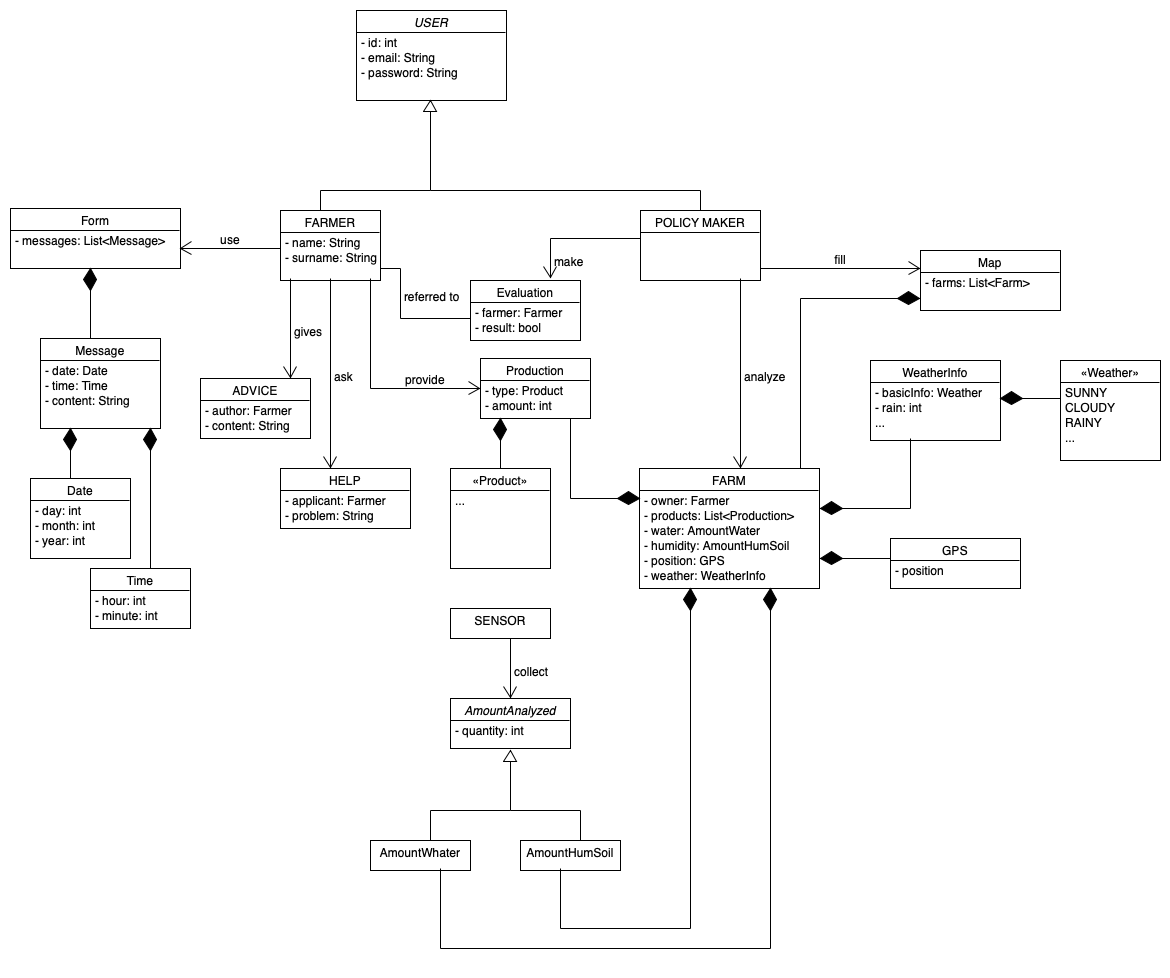
\includegraphics[width=1\textwidth]{images/UMLSW2_1.png}
    \caption{UML diagram.}
    \label{fig:uml}
    \end{center}
\end{figure}
\subsubsection{State Diagram}
\begin{figure}[H]
    \begin{center}
    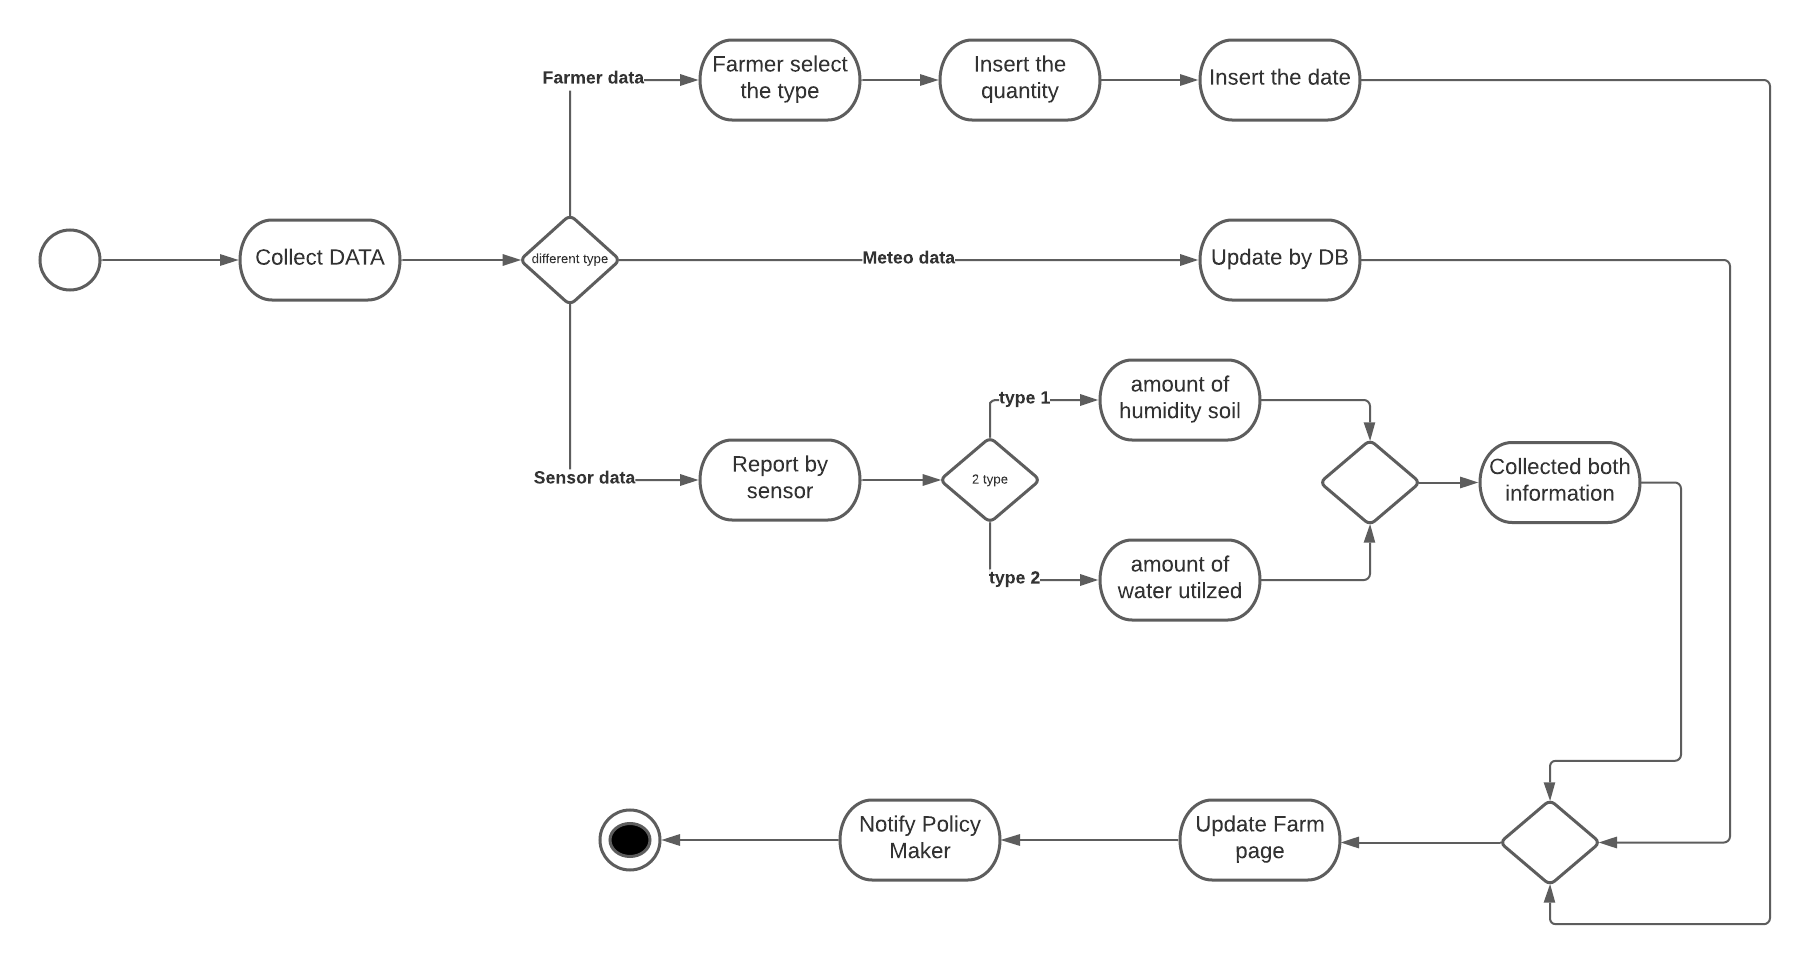
\includegraphics[width=1\textwidth]{images/State chart 1.png}
    \caption{Update Farmer page.}
    \label{fig:state1}
    \end{center}
\end{figure}
\begin{figure}[H]
    \begin{center}
    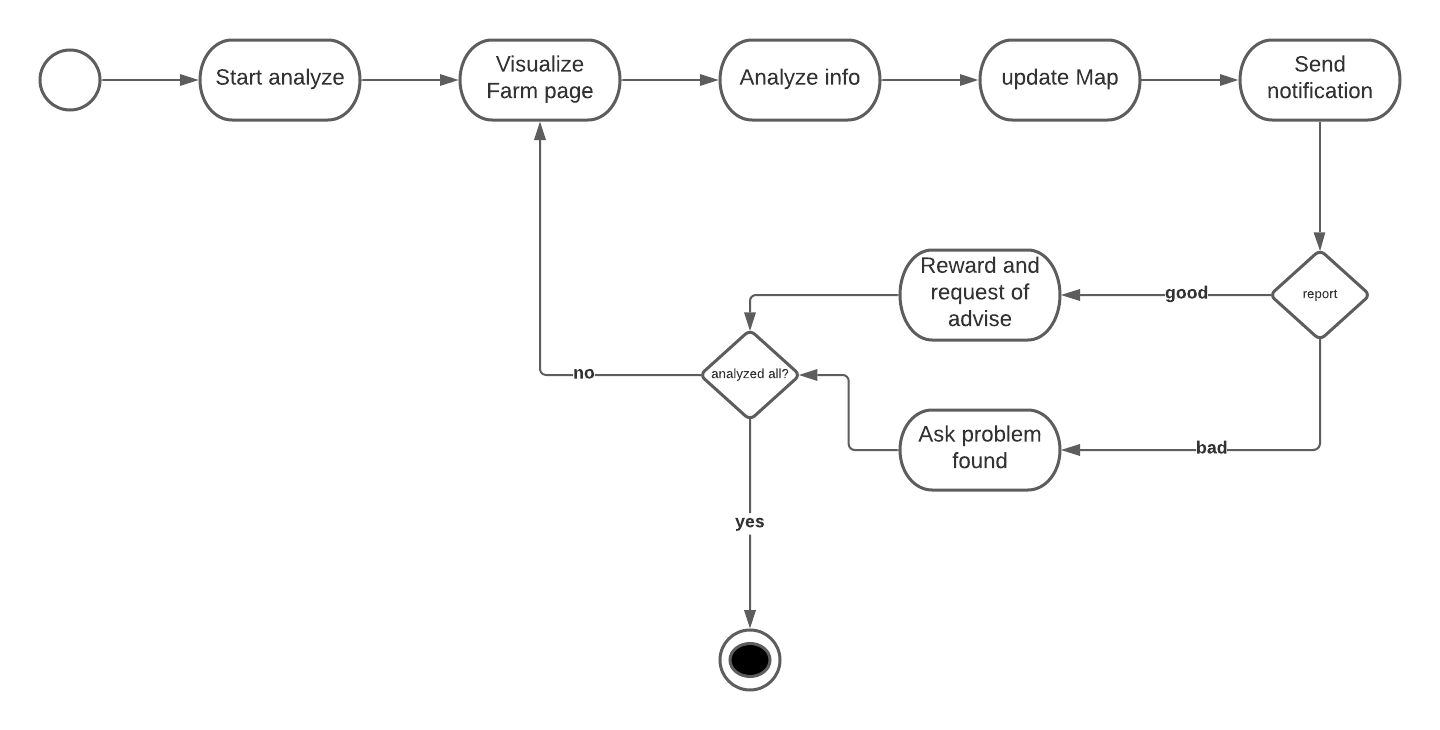
\includegraphics[width=1\textwidth]{images/State chart 2.png}
    \caption{Analysis of farmers.}
    \label{fig:state2}
    \end{center}
\end{figure}
\begin{figure}[H]
    \begin{center}
    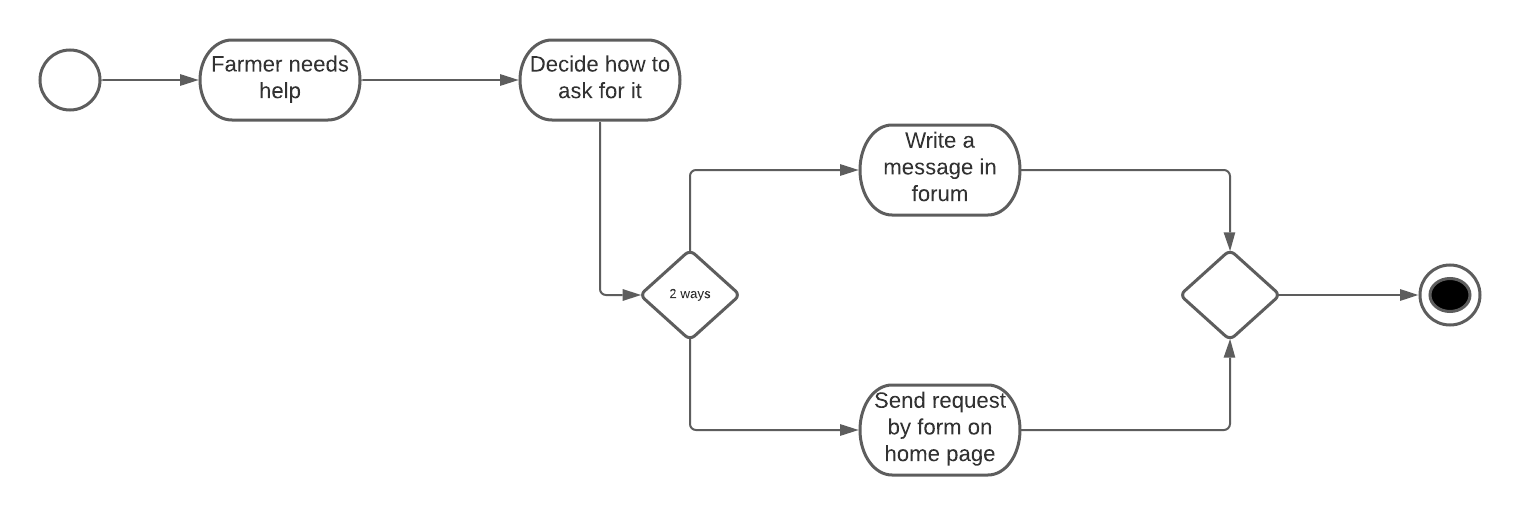
\includegraphics[width=1\textwidth]{images/State chart 3.png}
    \caption{Request of help.}
    \label{fig:state3}
    \end{center}
\end{figure}
\newpage
\subsection{Product Functions}
\label{subsection:2.2}
This section provides a summary of the main features and 
functions offered by the software regarding
the goals already described in section ~\ref{section:1.1.1}

In the following description it is important to highlight that both
the policy makers and the farmers must be logged in.

\subsubsection{Farmers insert data} 
This functionality is accessible to all farmers. 
The application provides a form in which the farmer can easily insert data of his/her production.
The form is easy to fill in, in order to complete it the farmer need to indicate:
\begin{itemize}
    \item the \textbf{type of product}
    \item the \textbf{amount} producted of the selected type
    \item the \textbf{date} relative to the date of the production
\end{itemize}
If the farmer needs to add more than one type of product, 
he/she can fill in the form multiple times.
After completing the form the user is redirected to the homepage and the policy makers 
can see the updated data.
This functionality can be done more than once a day since the farmer can select the date, 
so it is possible for him to insert data of past days too.
This operation can be repeated more than once a day since the farmer can select the date, so it is possible for him/her to insert data of past days too.



\subsubsection{Farmers visualize data}
This functionality lets the farmer visualize all the data 
acquired from the system. The farmer can visualize all data on his homepage.\\
The application shows:
\begin{itemize}
    \item meteorological  short-term and long-term forecast
    \item amount of water used by the farmer
    \item humidity of soil 
    \item personalized suggestions concerning specific crops to plant or specific 
    fertilizers to use – based on their location and type of production
\end{itemize}

\textbf{Should I say why he needs to visualize this data or how he uses it}


This functionality is always up to date, and does not need 
any input from the farmer.
It is used by the farmer only to have a general view of 
his farm and on how he could improve the productivity of his farm.



\subsubsection{Identify how farmers are performing}
The main features of the policy makers is to evaluate the work of each Farmer. 
In order to do that, they periodically analyze each farm page: 
the system allows them to visualize all the data in those pages 
(but not to modify it).
The analysis takes place twice a month.
With this analysis they classify the workers in two different way:
\begin{itemize}
    \item GOOD farmer : those how have been able to produce a significant amount of product with low resources, despite bad weather in that period.
    \item BAD farmer : those who did not produce much.
\end{itemize}
Policy makers inform each farmer the result they have achieved with a notification: 
\begin{itemize}
    \item GOOD farmers receive a special 
    incentive, and also a request to submit 
    from their personal web page some advice that could be useful to the others. 
    \item To BAD farmers is asked to submit an explicit request of help specifying the problems they had.
\end{itemize}
The system has a specific web page that allows all 
the users to look at a map of the area in which are 
specified all the farms. It is also shown if the farm's owner has performed 
a good job in that period.
At the end of each analysis the policy makers 
update the map (they are the only ones that are able to modify it).



\subsubsection{Interaction between farmers}
This functionality permits the farmers to comunicate with each other. 
The application has a specific web page were the farmers can send messages 
whenever they want.
If a farmer has an issue, before submitting a formal request of help to 
the policy makers 
by their home page, he can ask informally an advice by sending a message 
in the Forum.
It is not necessary to be a good farmer in order to answer someone elses 
message. All the messages are visible to everyone and 24h. 
Since it is an online application an internet connection is required to read or write 
on this page.



\subsection{Scenarios}
\subsubsection{Scenario 1}


\subsection{User Characteristics}
Dream has two different customers that need to be 
distinguished in order to provide the various 
features specified in subsection ~\ref{subsection:2.2}.
\subsubsection{Farmer}
- Can register on Dream in order to be recognized as farmer.\\
- Must log in on the website to use the services offered.\\
- Can discuss with other farmers.\\
- Is able to insert data about their daily production. \\
- Can ask for help to other farmers or to policy makers.\\
- Can retrieve data regarding weather forecast, water irrigation system or humidity of soil.\\
- Can look for advice of several products.\\
- Can check whether their performance is identified as good or bad.
\subsubsection{Policy Maker}
- Already has the credential to access to the system.\\
- Must login to Dream to benefit of its services.\\
- Can look all farms' pages.\\
- Can update the map.\\
- Can send suggestions to whom explicitly notices a problem.\\
- Can send notifications to the farmers.\\
- Decides the value of the incentive for the good farmers.\\
- Evaluates the performance of the farmers.\\



\subsection{Domain Assumptions, Dependencies and Constraints}
This subsection focuses on what it is assumed in order for our system to offer the services as expected.
Moreover it focuses on the limitations that the system could face.

\subsubsection{Domain Assumptions}
\textbf{DA1} In order to access the system users need to have Internet connection.\\
\textbf{DA2} Farmers always insert correct data on their production activity.\\
\textbf{DA3} Data from sensors is always correct.\\
\textbf{DA4} Date and Time on the system are always correct.\\
\textbf{DA5} The position of the Farm is always correct.\\
\textbf{DA6} Internet connection works always without errors.\\
\textbf{DA7} Meteorological data is accurate.\\
\textbf{DA8} Every farm has a different position.\\
\textbf{DA9} Each farm belongs to exacly one farmer.\\
\textbf{DA10} Discussion on the forum are related only to the farm activity.\\
\textbf{DA11} Formal request of help must be related to a farmer's own production.\\
\textbf{DA12} Advice on a product must be given by a farmer that produces the same type.\\
\textbf{DA13} Performances of farmers are always identified correctly.\\
\textbf{DA14} Farmers can insert data more than once a day.\\
\textbf{DA15 The username must be unique.}\\
\textbf{DA16} Policy Makers have a given username and password to access the system.

\subsubsection{Constraints}